\section{The First Direct Detection of Gravitational Waves}

Advanced LIGO's first observing run (O1) lasted from September 12, 2015 - 
January 19, 2016. In this observing run, the first direct detection of 
gravitational waves was achieved with the discovery of two binary black 
hole mergers, GW150914 and GW151226 \cite{GW150914-DETECTION,GW151226}. 
In total, 51.5 days of coincident analysis data were recorded in O1. 
After data with excess noise were removed from the analysis, the 
total amount of coincident data was 49.8 days.
%After category 1 vetoes were applied, the total coincident analysis 
%time was reduced to 50.3 days. After category 2 vetoes were applied, 
%the total coincident analysis time was reduced to 49.8 days. (??) 

Along with the publication detailing the first direct detection of 
gravitational waves, 12 companion papers were released 
that gave a complete description of the O1 analyses and the state 
of the interferometers during the run. A full list of these 
publications is available on the LIGO document control center 
(papers.ligo.org). 
Most relevant to this thesis are those that describe the CBC search 
in O1 \cite{GW150914-CBC}, the transient noise in the interferometers 
\cite{GW150914-DETCHAR}, and the 
overall state of the interferometers \cite{GW150914-DETECTORS}. 

\section{Foreground Events}

\subsection{GW150914}

The first signal discovered in O1, GW150914, marked the first 
direct detection of gravitational waves.
Figure \ref{fig:GW150914} shows a 
filtered time domain representation of the first detection, 
GW150914, with the best estimated 
waveform overlaid on top. Both the signal and the waveform have been 
bandpass filtered to isolate the frequency range where the signal has 
power. Static lines, such as the 60 Hz power line frequency and 
interferometer calibration lines, have been notched out of the data. 
The signal demonstrates the characteristic ``chirp", 
increasing in frequency and amplitude as a function of time as  
expected from a compact binary coalescence. 

\begin{figure}[ht!]
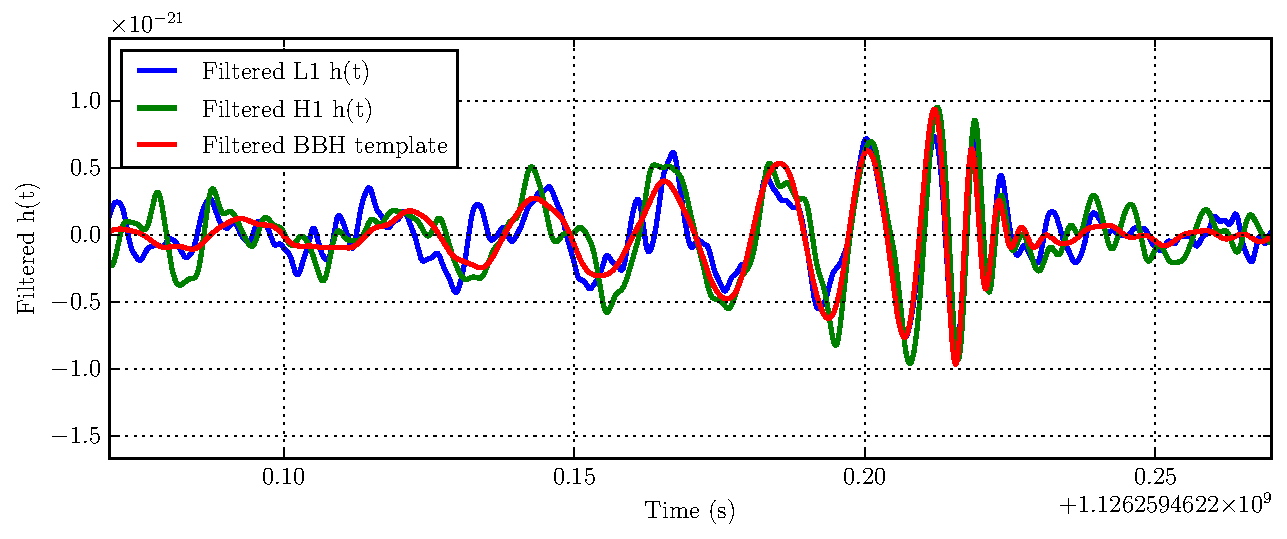
\includegraphics[width=\textwidth]{figures/O1/GW150914-timeseries}
\caption[GW150914 timeseries]{Time domain representation of H1 and L1 %
        gravitational wave strain at the time of GW150914. The blue %
        and green curves are detector strain, $h(t)$, zero-phase bandpass %
        filtered to isolate the %
        frequencies that contain signal. The red curve is a CBC waveform %
        generated using the best estimated parameters. The CBC waveform %
        has been filtered in the same way as the strain curve. The overlap %
        between the three curves is significant, demonstrating many cycles %
        of clear coherence and demonstrating the expected 'chirp' signal.}
\label{fig:GW150914}
\end{figure}

It is exceptional that GW150914 is visible in the detector data with 
very conservative filtering. Due to the high total mass of the system, 
which is detailed in Table \ref{table:foreground}, the black holes 
of GW150914 coalesced quickly and at a low frequency, spending about 
0.2 seconds in the frequency range that aLIGO is sensitive to. The 
signal was also tremendously loud due to its total mass and relatively 
close distance. 
As a result, the power in the signal is highly localized in time, 
producing a short, loud waveform that is readily visualized.
A discussion of the data validation process relevant to GW150914 is 
found in Section \ref{sec:GW150914-validation}.

\subsection{GW151226}

The other binary black hole signal discovered in O1, GW151226, has a rather different 
morphology. The system that produced GW151226 was roughly three times 
less massive than that of GW150914 and was estimated to have merged 
at a similar distance (see Table \ref{table:foreground}). Due to the 
lower total mass, GW151226 has an overall lower amplitude than GW150914 
and has its power distributed more broadly in time. GW151226 spent about 
2 seconds in the frequency band that aLIGO is sensitive to, which is a 
factor of 10 longer than the duration of GW150914. For these reasons, 
it is not feasible to generate a time domain visualization of the signal. 
However, this is a fantastic demonstration of the value of a 
matched-filter search for CBC signals. The signal-to-noise ratio 
reported by a matched-filter search is an 
integral in the frequency domain that is designed to identify modeled 
signals regardless of their duration.

\subsection{LVT151012}

The third loudest foreground event in the analysis, LVT151012, stands out 
from the background distribution but is not statistically significant 
enough to be labeled as a gravitational wave detection. Its statistical 
significance is calculated to be just under $2\sigma$. While it is not 
being claimed as a gravitational wave detection, there is no obvious 
reason to believe that it is a noise artifact based on detector 
performance. It is possible that LVT151012 is part of a larger 
population of gravitational waves that is expected to contain 
quiet, threshold signals as well as clear detections.

\begin{table}[ht!]%
  \begin{center}
    \footnotesize
    \begin{tabular}{ccccccc}
    \hline
    Event & Time(UTC) & FAR ($yr^{-1}$) & $m_1$ ($M_{\odot}$) & $m_2$ ($M_{\odot}$) & 
    $\chi_{eff}$ & $D_L$ (Mpc) \\
    \hline
    GW150914 & \begin{tabular}{@{}c@{}}14 September \\ 2015 \\ 09:50:45 \end{tabular} & 
    $< 5.8\times10^{-7}$ & $36_{-4}^{+5}$ & $29_{-4}^{+4}$ & $-0.06_{-0.18}^{+0.17}$ & 
    $410_{-180}^{+160}$ \\
    GW151226 & \begin{tabular}{@{}c@{}}26 December \\  2015 \\ 03:38:53 \end{tabular} & 
    $< 5.8\times10^{-7}$ & $14_{-3}^{+9}$ & $8_{-3}^{+2}$ & $0.20_{-0.10}^{+0.21}$ & 
    $490_{-210}^{+180}$ \\
    LVT151012 & \begin{tabular}{@{}c@{}}12 October \\ 2015 \\ 09:54:43 \end{tabular} & 
    0.44 & $23_{-5}^{+18}$ & $13_{-5}^{+4}$ & $0.0_{-0.2}^{+0.3}$ & 
    $1100_{-500}^{+500}$ \\
    \hline
    \end{tabular}
  \end{center}
  \caption[Table of foreground events]{Table of foreground events found in the first %
           observing run. %
           The quoted false alarm rates are calculated by the PyCBC search pipeline. %
           The GstLAL search pipeline reported similar results. % 
           Two binary black hole systems, GW150914 and GW151226, were %
           discovered with a false alarm rate $< 5.8\times10^{-7}$, which is the upper %
           limit on false alarm rate set by the amount of time used in the analysis. %
           This corresponds to a statistical significance $> 5.3\sigma$. %
           A third event, LVT151012, was an interesting foreground event that was not %
           statistically significant to be claimed as a detection, but could be part %
           of a larger gravitational wave population that includes weaker signals.
           } 
  \label{table:foreground}
\end{table}

\section{Background Noise}

To estimate the stability of the background noise used in the O1 
analysis, the time period of September 12 - October 20, 2015 is 
studied. This is the stretch 
of time used for an extended background analysis of GW150914. 

The first 
visualization of background noise stationarity is the amplitude 
spectral density (ASD) of $h(t)$. Figure \ref{fig:median-asd} 
shows the 
median ASD of the detector data from each interferometer over this 
time period as a function of frequency. The shaded regions indicate 
the 5th and 95th percentile in that particular frequency bin. 
The most noticeable feature is the variance in the low frequency 
noise at L1, which was not fully understood at the end of the run. 
Most of this variance is below 30 Hz, which is the 
low frequency cutoff used in the matched filter search, and would 
not have an effect on the output of the CBC search. The L1 data 
also had a higher variance in the 60-200 Hz region, which was a 
limiting noise in the PyCBC analysis (??). Other than these two regions, 
the spectra appear to be consistent and have reasonable variance 
at all frequencies \cite{GW150914-DETCHAR}.

\begin{figure}[ht!]%
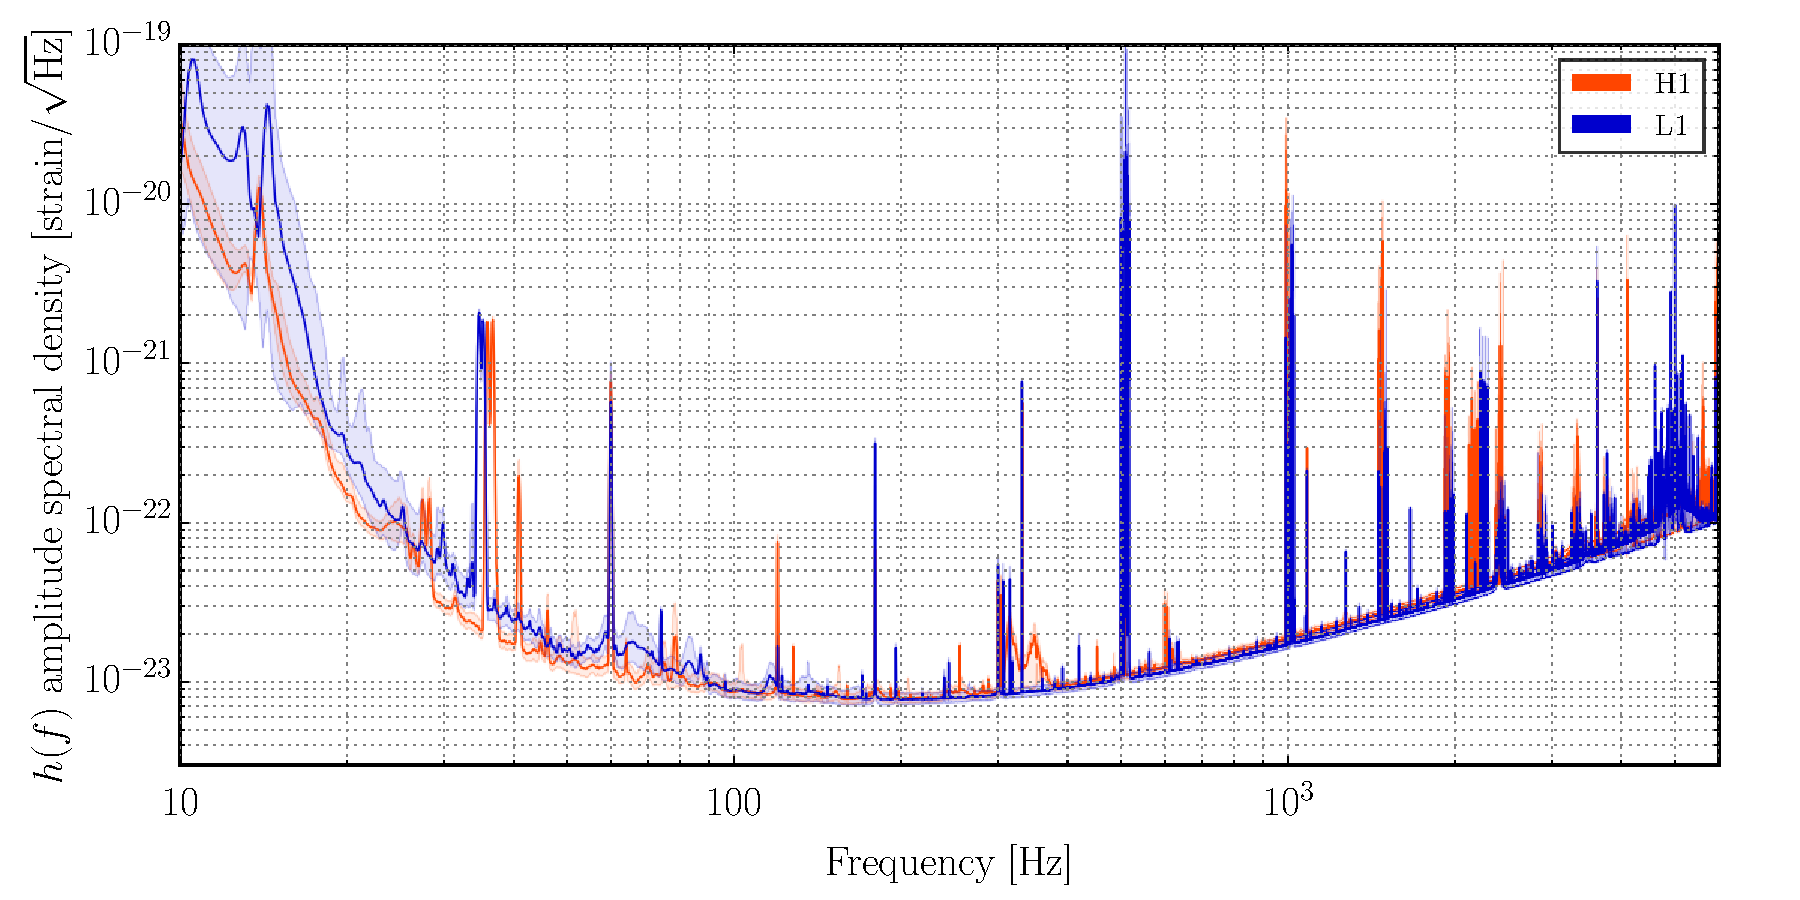
\includegraphics[width=0.85\textwidth]{figures/O1/H1L1-OBSERVING_GW150914_PERCENTILE_SPECTRUM-1126073342-3309798}
\caption[Median noise ASD in O1]{Median noise amplitude spectral density %
         in the first analysis period of O1. The shaded regions indicate %
         the 5th and 95th percentile in a given frequency bin. The background %
         for H1 was very stable throughout the run, which very few high %
         variance bins. The background at L1 showed deviations from the %
         median behavior in two regions: below 30 Hz and between 50-200 Hz. %
         The strong lines in the noise spectrum are due to injected calibration %
         lines, environmental sources such as the 60 Hz power line harmonics, %
         and mechanical resonances.
         }
\label{fig:median-asd}
\end{figure}

A useful figure of merit for detector noise stationarity is the 
inspiral range. This is the distance at which a given source 
of gravitational waves 
could be recovered at SNR 8 in current detector noise assuming 
optimal orientation and sky location. Since GW150914 is the 
centerpiece of the analysis, the inspiral range was calculated using 
its parameters as the gravitational wave source. Figure \ref{fig:inspiral-range} 
shows 
the inspiral range over the time used for an extended background 
analysis of GW150914. The inspiral range was between 1500-2000 Mpc 
for both instruments throughout the run. The L1 data, with the 
previously mentioned fluctuations, were slightly less sensitive to 
gravitational wave signals throughout the run. The two vertical lines 
represent GW150914 (dashed) and LVT151012 (dash-dotted) \cite{GW150914-DETCHAR}.

\begin{figure}[ht!]%
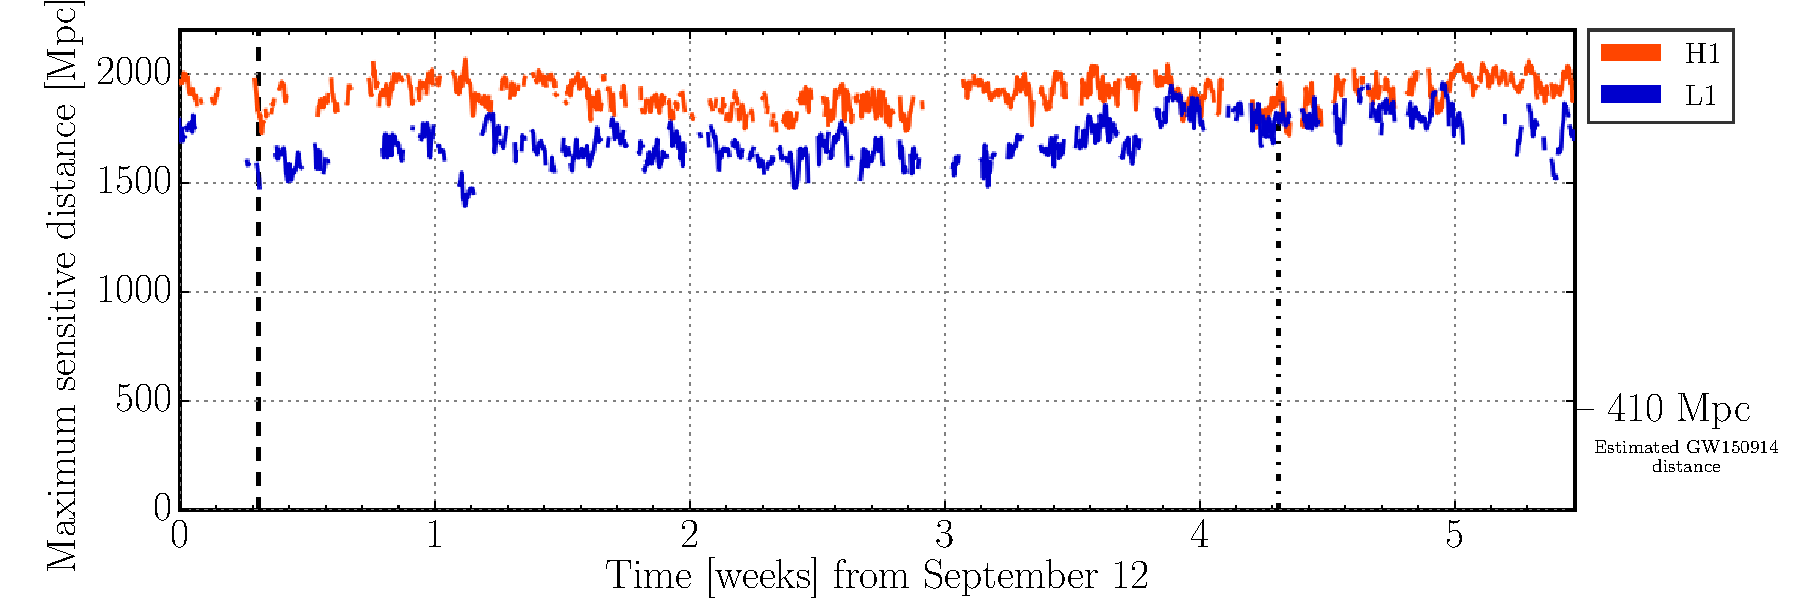
\includegraphics[width=0.85\textwidth]{figures/O1/inspiral-range}
\caption[Inspiral range in O1]{Inspiral range for sources with %
         the same parameters as GW150914. This is the distance at %
         which a signal could be recovered at SNR 8 given optimal %
         orientation and sky position. The inspiral range for %
         GW150914-like sources was stable through the first analysis %
         period of O1. The inspiral %
         range for H1 was typically higher due to noise fluctuations %
         at L1. Overall, the inspiral range was between 1500 - 2000 Mpc. %
         Each data point was calculated using a 2048 second stride. %
         For reference, GW150914 is estimated to have been generated at a %
         distance of 410 Mpc. %
         }
\label{fig:inspiral-range}
\end{figure}

The final figure of merit for establishing that the detector noise was 
stationary is to look at the rate of events, or 'triggers', produced by the PyCBC pipeline 
between September 12 - October 20, 2015. 
Figure \ref{fig:pycbc-rate} shows 
the rate of single 
interferometer triggers produced by PyCBC for both H1 and L1 in this time 
span. The circles indicate the rate of triggers with a re-weighted SNR 
$\geq 6.5$. The crosses indicate the rate of triggers with a re-weighted SNR 
$\geq 8$, which represents the rate of loud, non-Gaussian triggers in the 
analysis. The overall rate of triggers was consistent throughout the 
observing run, typically reported between 0.1 - 1.0 Hz. The rate of triggers 
with a re-weighted SNR $\geq 8$ was typically $< 0.01$ Hz. The dashed 
and dash-dotted lines indicate the times of GW150914 and LVT151012 respectively 
\cite{GW150914-DETCHAR}. 

\begin{figure}[ht!]%
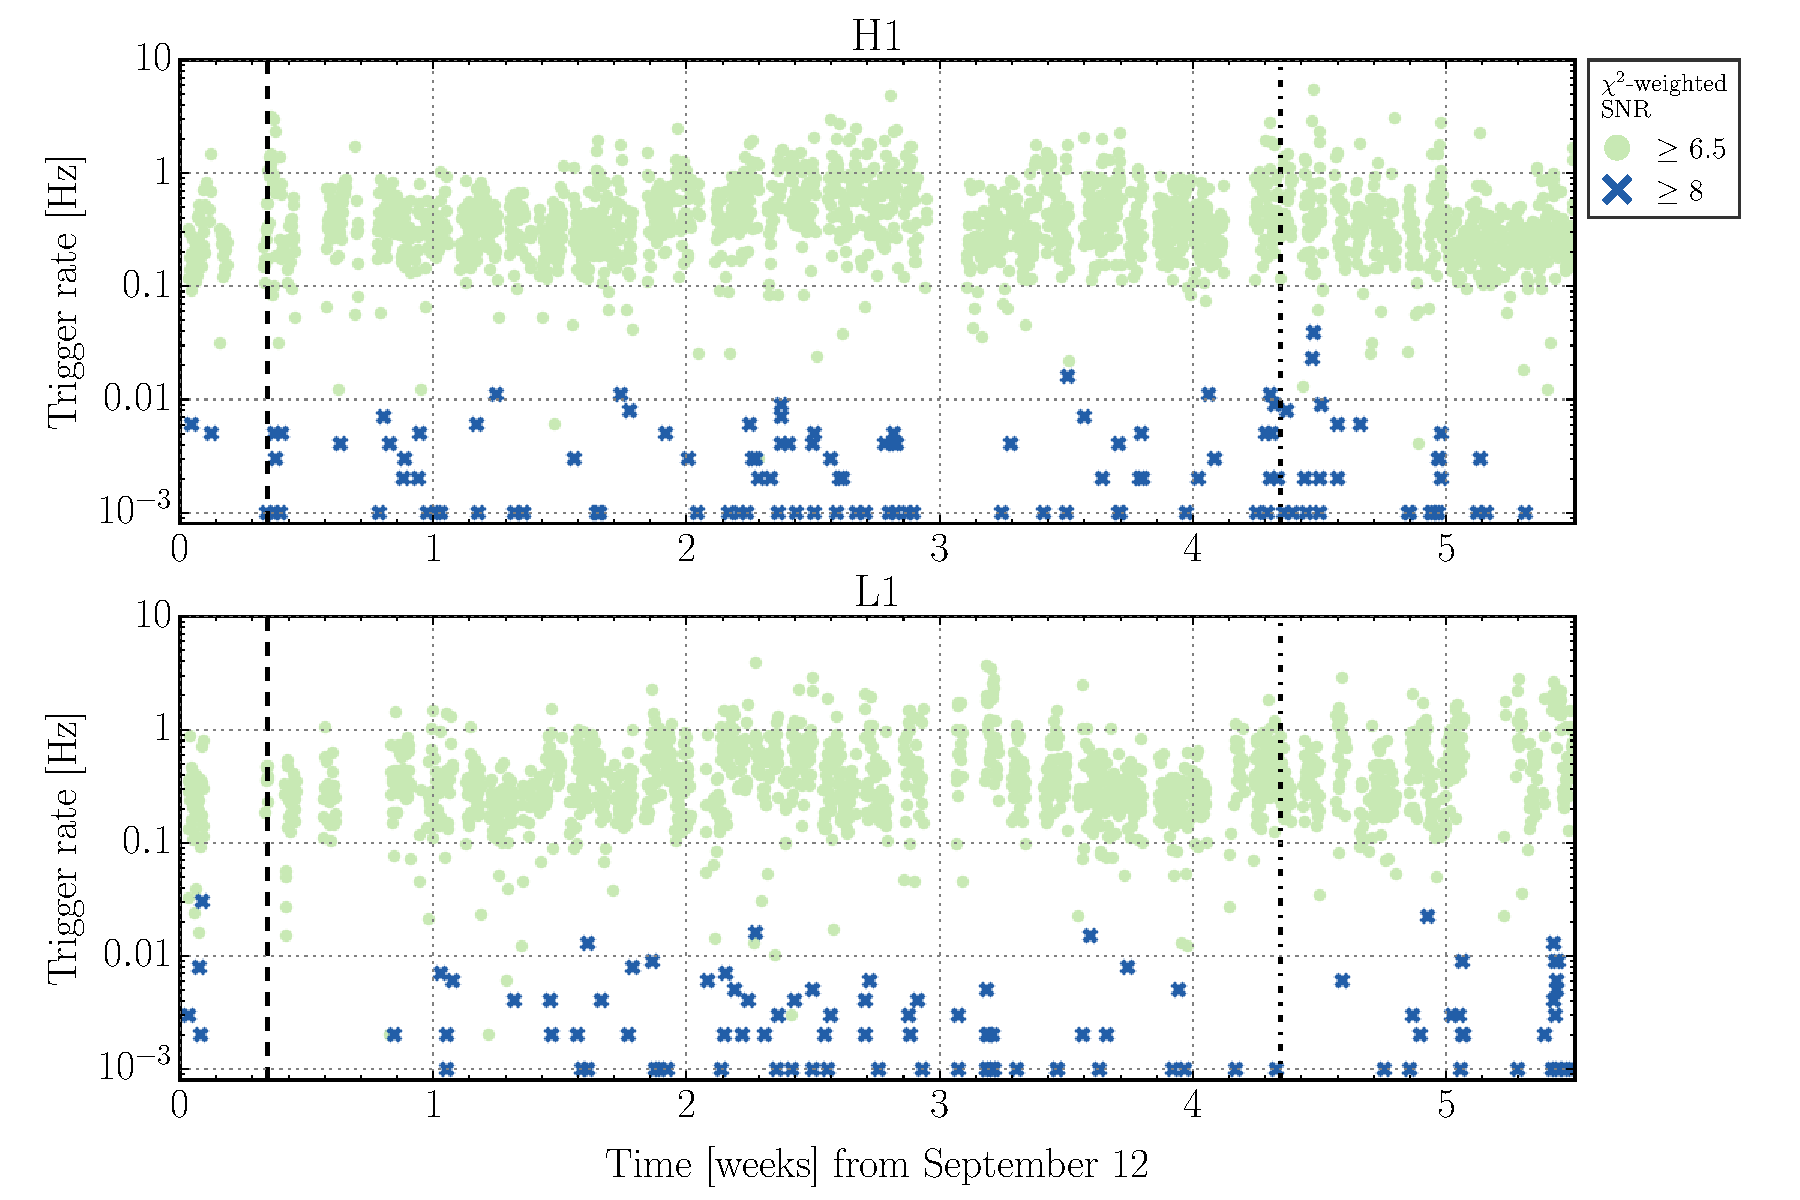
\includegraphics[width=0.85\textwidth]{figures/O1/pycbc-rate-versus-time}
\caption[PyCBC trigger rates in O1]{PyCBC single interferometer background trigger %
         rates in O1. For these rates, any triggers found in coincidence %
         were removed from the data set. Rates were calculated over a 2048s stride. %
         The rate of triggers with %
         re-weighted SNR $\geq 6.5$ was stable throughout the analysis, typically %
         reported at 0.1 - 1.0 Hz. The rate of louder triggers, at re-weighted SNR %
         $\geq 8$, was typically at $< 0.01$ Hz. The dotted and dash-dotted lines %
         represent the times of GW150914 and LVT151012 respectively.
         }
\label{fig:pycbc-rate}
\end{figure}

\section{CBC Results}

The search for compact binary
coalescences was performed by two parallel search pipelines: PyCBC and 
GstLAL. In addition to these searches for modeled sources, an unmodeled 
burst search, Coherent Wave Burst (CWB), was run to search for coherent 
transient signals in the two Advanced LIGO interferometers. 
All three of these analyses produced consistent results. 
For brevity, we will focus on the results of the PyCBC search pipeline.

Figure \ref{fig:pycbc-hist-gw150914} shows the results of the PyCBC search 
over the whole of the first observing run. The black curve shows the 
number of expected foreground events at a given $\hat{\rho_c}$ based on 
background noise alone for the analysis. For this curve, GW150914 is 
allowed to remain in the data when generating a background from timeslides. 
This answers an interesting question: if GW150914 is considered to be a 
chance coincidence due to noise, could a combination of GW150914 in 
one detector and background noise in the other detector generate a 
signal as loud is GW150914?

The orange squares indicate the 
number of foreground events that were actually recovered by the search 
pipeline. The false alarm rate for a given foreground 
event is defined as the rate of background events with a $\hat{\rho_c}$ 
greater than or equal to that of the foreground event. GW150914 
was an exceptionally loud signal and is the loudest event in the 
analysis. Since there are no background events as loud as GW150914, 
its statistical significance has a lower limit of $5.3\sigma$ 
but is not exactly calculated. The associated statistical significance 
is listed on the horizontal bars on the top of the plot. The color 
of each bar corresponds to the background from which the statistical 
significance was measured.  

The blue curve shows the search background when GW150914 is removed 
from the analysis and not used when generating a background from 
timeslides. Since we believe that GW150914 is a real gravitational wave 
signal, using it in background calculations no longer provides a 
search background that is a realization of detector noise alone 
when evaluating the significance of quieter signals. 
If GW150914 is allowed to produce background events, the 
significance of GW151226, which is represented by the orange square at 
$\hat{\rho_c} = 12.6$, is highly diminished. This can be seen by comparing 
the blue and black curves. The differences between them, including the 
extension of the background to $\hat{\rho_c} = 21$ , are the result 
of GW150914 combining with background noise.

\begin{figure}[ht!]%
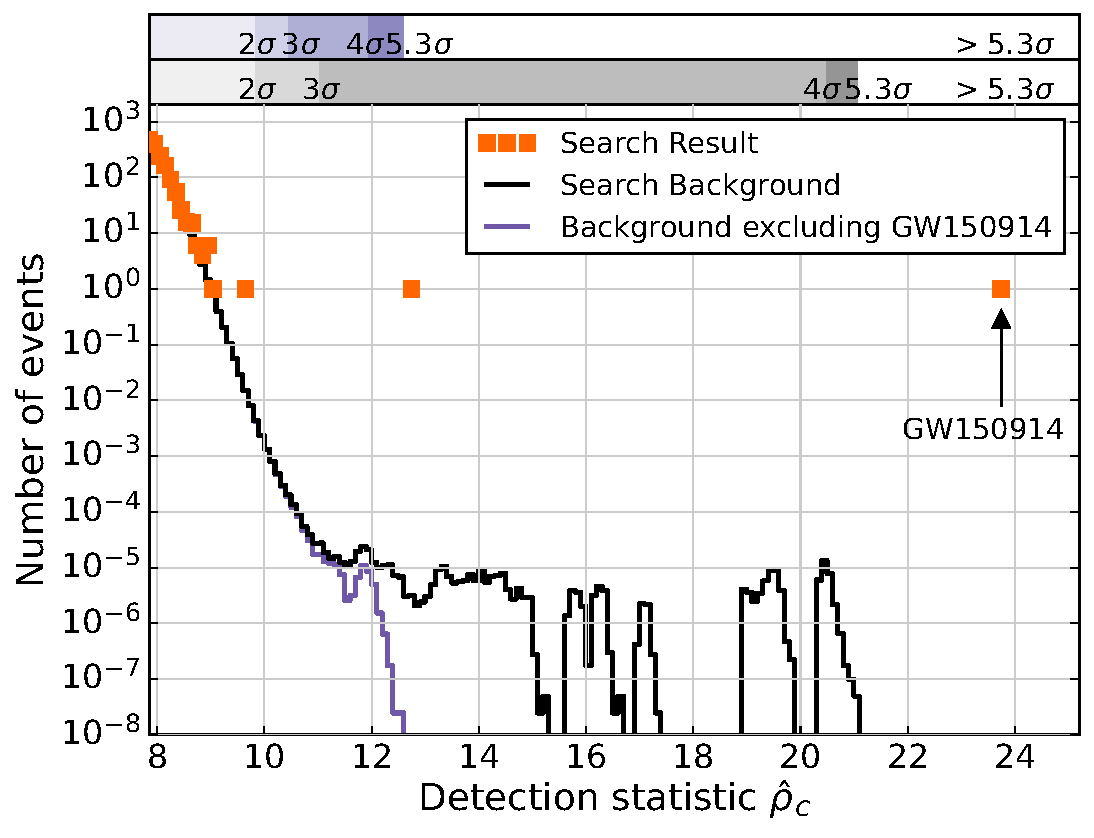
\includegraphics[width=0.85\textwidth]{figures/O1/pycbc_hist_GW150914}
\caption[PyCBC result histograms for GW150914]{PyCBC search results for %
         the first observing run. The black curve is the search background %
         relevant to GW150914. The blue curve is the search background %
         relevant to GW151226 where GW150914 has not been included in the %
         search background calculation. GW150914 was the loudest event in %
         the first observing run and was reported with a significance %
         $> 5.3\sigma$. Figure \ref{fig:pycbc-hist-gw151226} provides % 
         a better visualization of the significance of GW151226.}
\label{fig:pycbc-hist-gw150914}
\end{figure}

With GW150914 removed from the search background, we can correctly evaluate the 
statistical significance of GW151226. 
Figure \ref{fig:pycbc-hist-gw151226} shows a zoomed in version
of the search background with GW150914 removed. 
GW151226 is the loudest event in the analysis once GW150914 and its associated 
background triggers have been removed. Since there are no background events 
as loud as GW151226, its false alarm rate can be bounded to 1 per the entire 
analysis time. The associated statistical significance has a lower limit of 
$5.3\sigma$ but can not be directly calculated. The blue curve in this plot 
shows the search background with GW151226 removed from the analysis. Any 
quieter foreground triggers, such as LVT151012, will have their false alarm 
rate and statistical significance determined by this background distribution.  
LVT151012, which is the second loudest foreground event in Figure 
\ref{fig:pycbc-hist-gw151226}, was recovered at $\hat{\rho_c} = 9.6$ and 
assigned a statistical significance of just under $2\sigma$.  

\begin{figure}[ht!]%
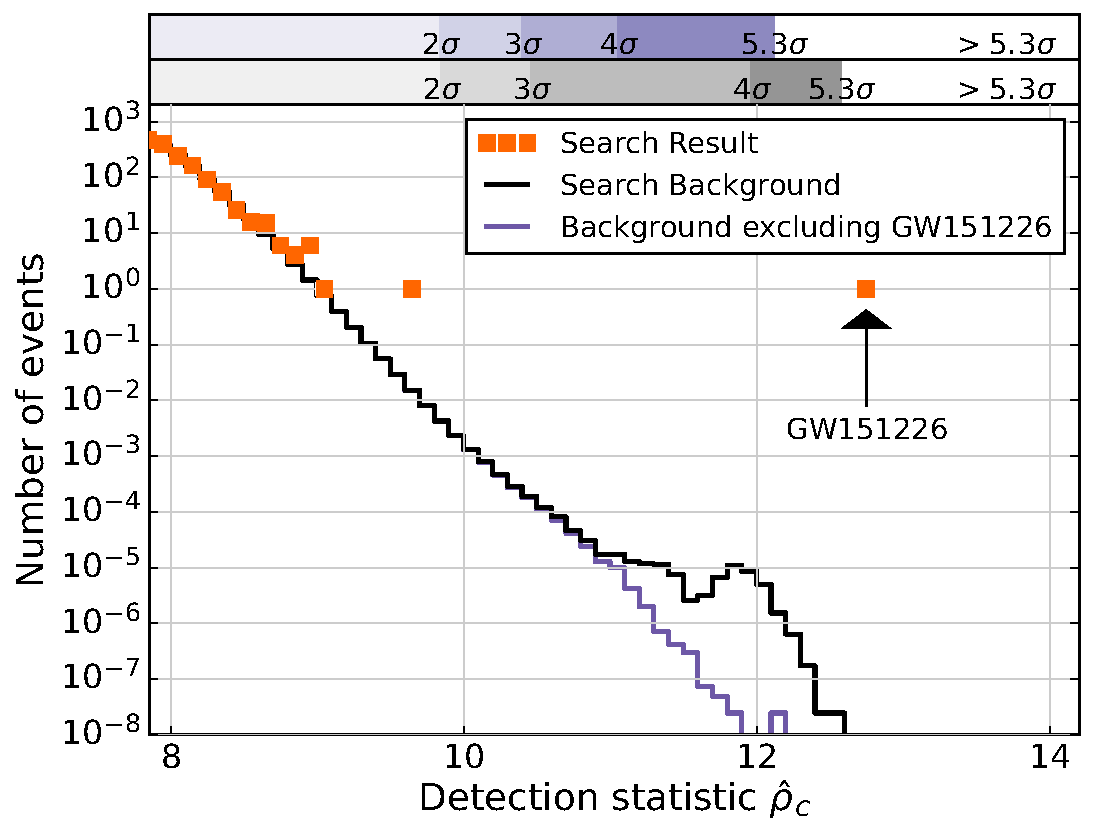
\includegraphics[width=0.85\textwidth]{figures/O1/pycbc_hist_GW151226}
\caption[PyCBC result histograms for GW151226]{PyCBC search results for the %
         first observing run with GW150914 removed. The black curve is the %
         complete search background. The blue curve is the search background %
         when GW151226 is removed and not allowed to combine with noise to %
         generate background events. In both cases, GW151226 is the loudest %
         event in the analysis. The statistical significance of GW151226 %
         is bounded to be $> 5.3\sigma$. The second loudest event in this %
         plot is LVT151012, which is assigned a statistical significance of %
         just under $2\sigma$.}
\label{fig:pycbc-hist-gw151226}
\end{figure}

\section{Summary}

The data used in the first observing run were stationary on a scale of 
weeks, as evidenced by the lack of variance in the noise amplitude 
spectral density, the stable background trigger rate, and the stable 
inspiral range.

The search results of the first observing run are summarized in Table 
\ref{table:foreground}. False alarm rates are quoted as estimated by the 
PyCBC search pipeline.  
The two discovered binary black hole signals, GW150914 and GW151226, differed 
by about a factor of 3 in total mass, which is responsible for the higher SNR  
of GW150914. Both events are estimated to have occurred at similar distances, 
with their error regions having significant overlap. 
The third interesting foreground event,
LVT151012, is estimated to have a total mass greater than GW151226, but its
distance is estimated to be much further away.

The estimated distance for 
GW150914, 410 Mpc, corresponds to 1.3 billion light years. Since general 
relativity predicts that gravitational waves travel at the speed of light, 
this means that the signal we measured as GW150914 was emitted 1.3 billion 
years ago, before complex life existed on Earth. For reference, 
the Andromeda Galaxy is less than 1 Mpc away from Earth. 

Both GW150914 and GW151226 were the loudest events when compared to their 
respective background distributions, resulting in a false alarm rate 
$< 5.8\times10^{-7} yr^{-1}$, which corresponds to a statistical significance of 
$> 5.3\sigma$. LVT151012 has a false alarm rate of $0.44 yr^{-1}$, which 
corresponds to a statistical significance of just under $2\sigma$.

